% -----------------------------------------------------------------------
% CHAPITRE 2 - DONNEES & METHODES (Boeny, Dynamic World 10 m -> 250 m)
% -----------------------------------------------------------------------
% A inclure dans votre .tex principal avec \input{chapitre2_donnees_methodes.tex}.
% Chiffres coherents avec chapitre3_resultats_clustering.tex (K=6, lissage 2,0%).
% Reproducibilite : SEED=1, random_state=1, nstart=25, TAILLE_SILHOUETTE=5000.
% -----------------------------------------------------------------------

\chapter{Données et méthodes}
\label{ch:donnees_methodes}

\section{Région d'étude : le Boeny (nord-ouest de Madagascar)}

\begin{figure}[H]
\centering
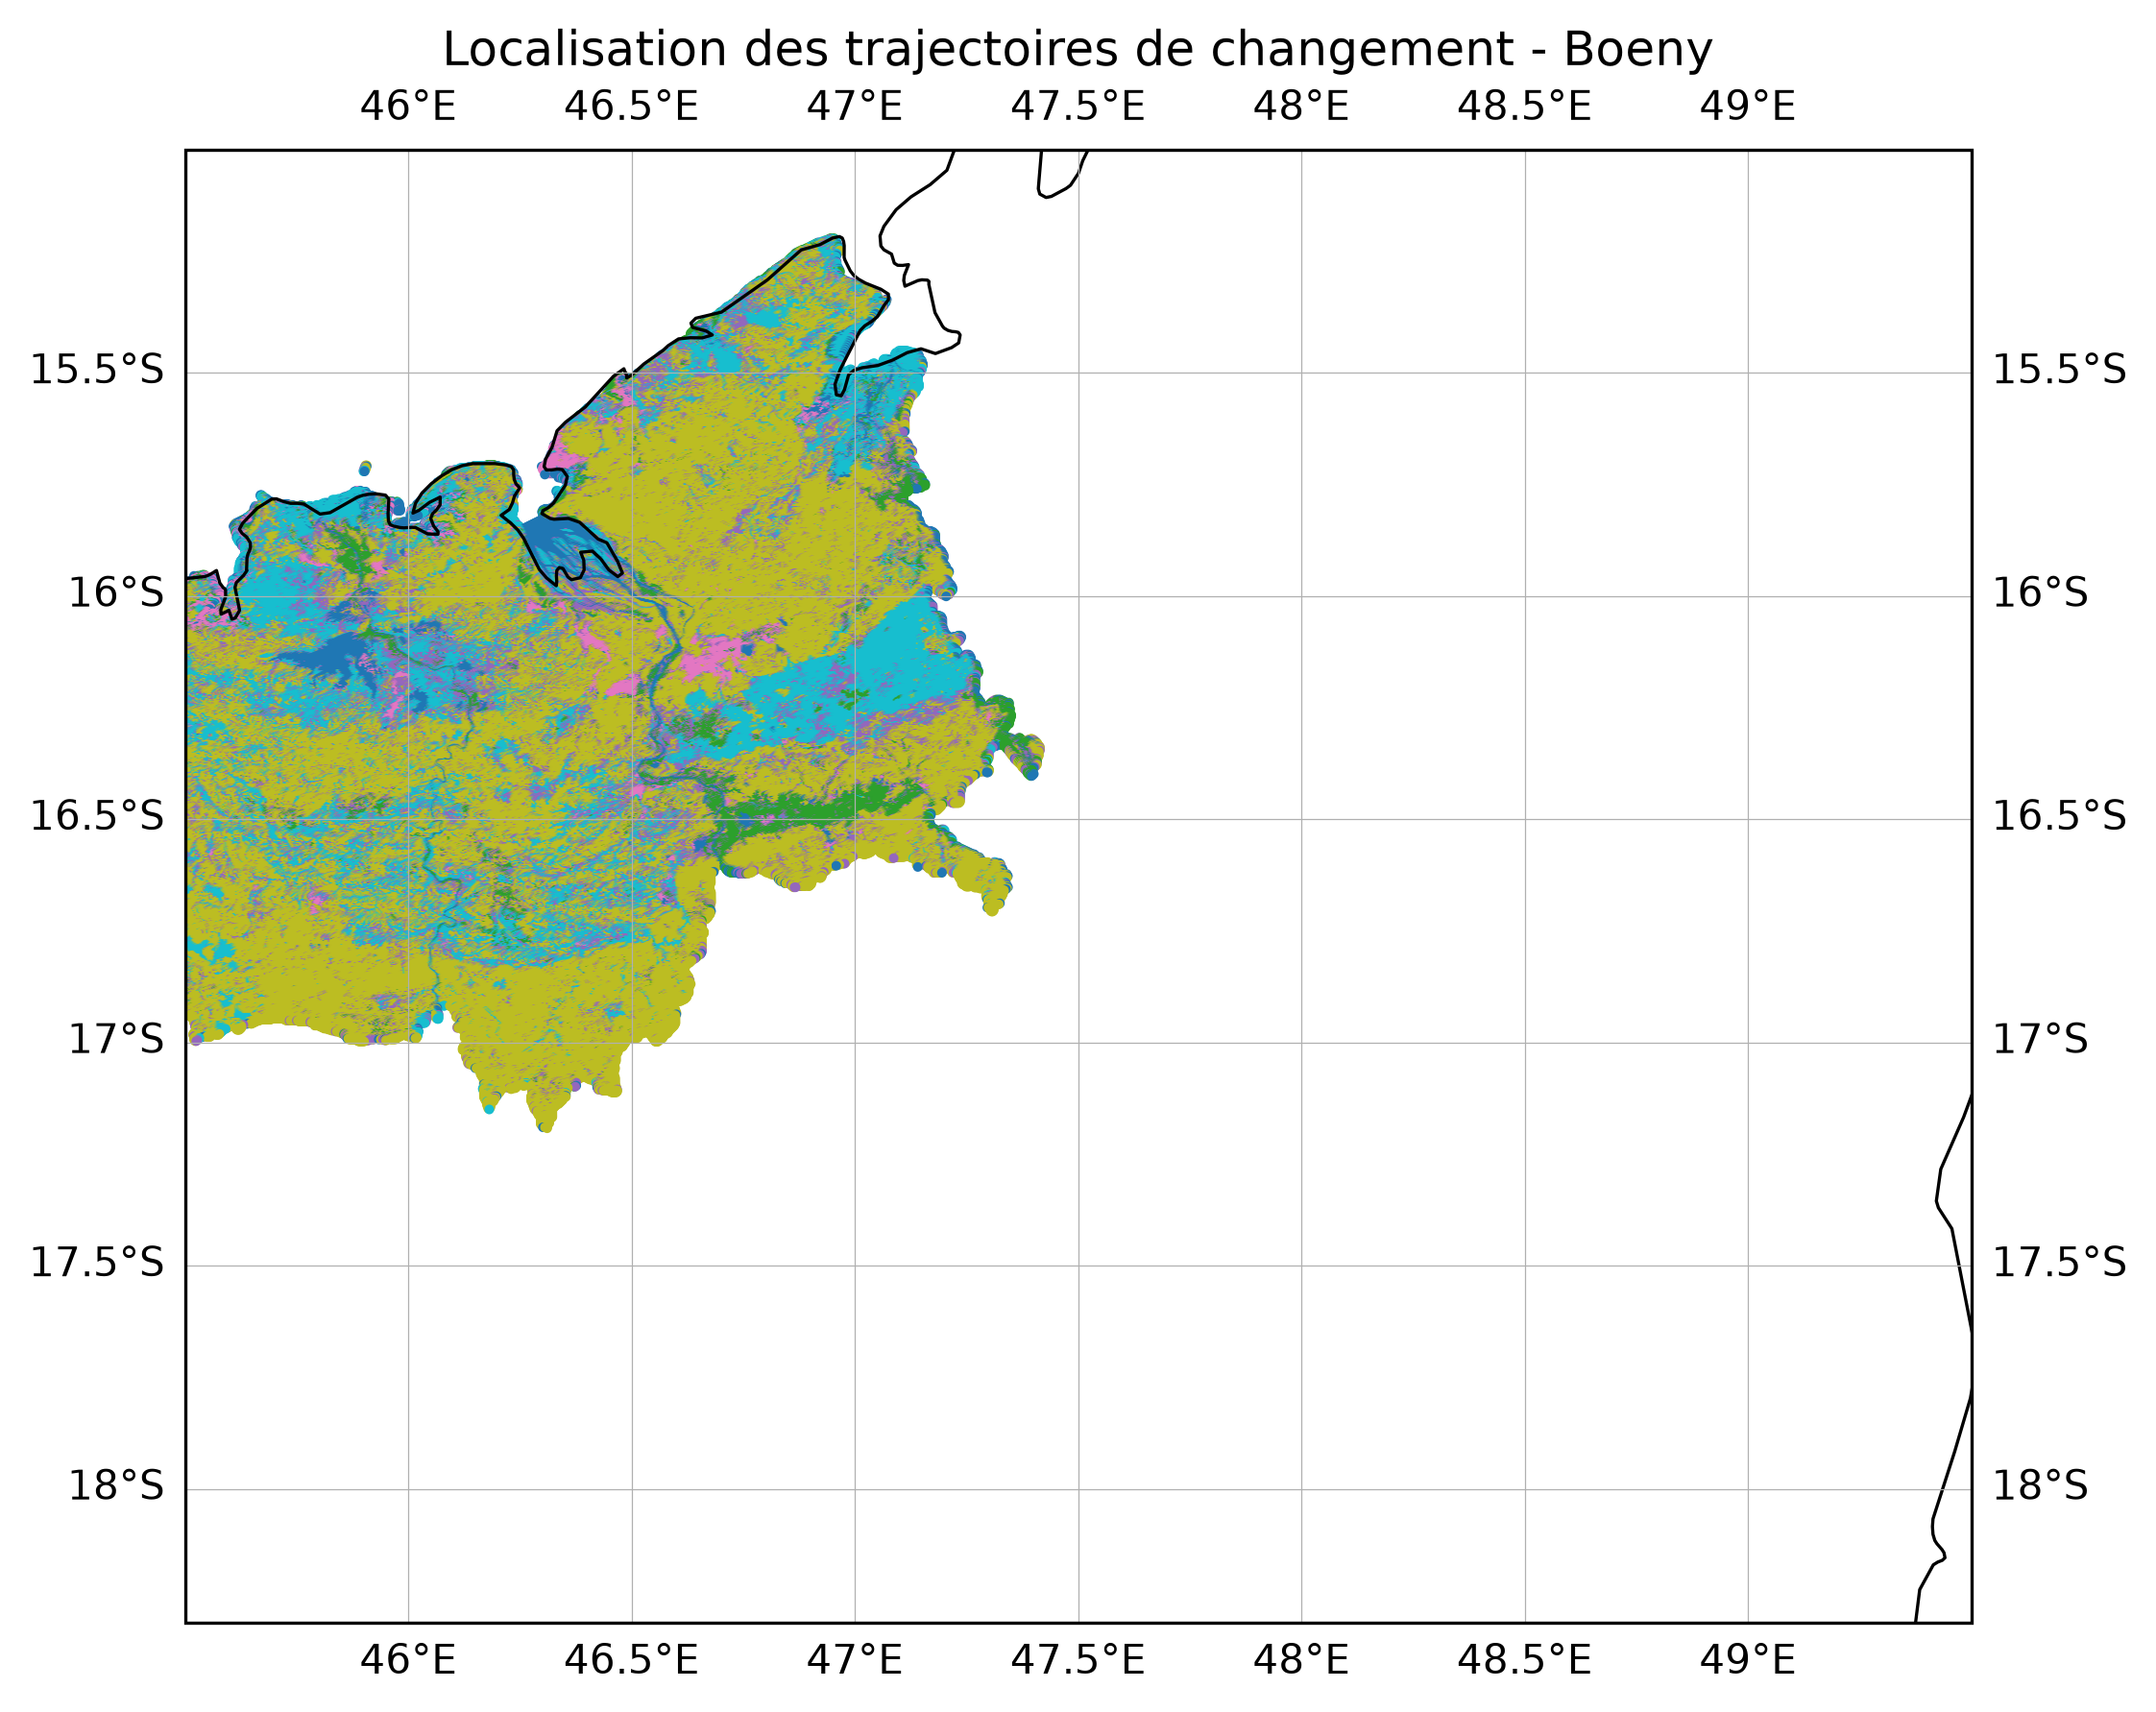
\includegraphics[width=0.85\textwidth]{carte_contexte_boeny.png}
\caption{Localisation du Boeny dans le nord-ouest de Madagascar.}
\label{fig:contexte_boeny}
\end{figure}

\paragraph{Situation.} Le Boeny est l'une des 23 régions de Madagascar, située
au nord-ouest du pays, bordée à l'ouest par le canal du Mozambique et traversée
par l'estuaire de la Betsiboka — l'un des plus grands estuaires de l'océan
Indien, célèbre pour ses eaux rouges chargées en sédiments. La région couvre
environ \SI{31}{\kilo\metre\squared} et se caractérise par un climat tropical
semi-aride (saison sèche marquée de mai à octobre, saison humide de novembre à
avril). Ces conditions favorisent un paysage en mosaïque : forêts sèches,
savanes arborées, cultures (principalement riz, maïs et manioc) et vastes
vasières estuariennes.

\paragraph{Intérêt pour l'étude.} Le Boeny combine en un même espace des
milieux parmi les plus stables (forêts sèches, savanes) et parmi les plus
dynamiques (estuaire de la Betsiboka, fronts pionniers agricoles). C'est un
territoire idéal pour analyser des \emph{trajectoires} de changement car il
concentre, sur une surface restreinte et homogène climatiquement, une grande
diversité de dynamiques.

\section{Données : Dynamic World (Google Earth Engine)}

\subsection{Source et caractéristiques}

\begin{table}[H]
\centering
\caption{Caractéristiques de la source de données Dynamic World.}
\label{tab:caracteristiques_dynamicworld}
\begin{tabular}{ll}
\toprule
\textbf{Caractéristique} & \textbf{Valeur} \\
\midrule
Fournisseur & Google (via Google Earth Engine) \\
Produit & Dynamic World (DW) \\
Résolution native & \SI{10}{\metre} \\
Période & 2016--2025 (10 ans) \\
Pas temporel & Annuel (mode d'occupation dominante) \\
Classes & 7 (eau, forêt, vég. non forestière, vég. inondée, cultures, bâti, sol nu) \\
Projection d'export & UTM 38S (EPSG 32738) \\
Accès & GEE — gratuit pour la recherche \\
\bottomrule
\end{tabular}
\end{table}

\paragraph{Justification du choix.} Dynamic World fournit une couverture
globale de l'occupation du sol à \SI{10}{\metre}, mise à jour dès 2016, avec
une nomenclature adaptée à l'analyse des zones humides et des fronts agricoles.
Son pas annuel sur 10 ans (2016--2025) est exactement la fenêtre d'observation
nécessaire à la détection des trajectoires de changement, y compris les
allers-retours (ex. eau $\leftrightarrow$ sol nu dans l'estuaire).

\subsection{Export et prétraitement}

Les images Dynamic World 2016--2025 (10 classes = 7 classes d'occupation +
classes « brouillard », « nuage », « eau ») sont exportées depuis Google Earth
Engine via le script \texttt{dynamicworldBoeny.py}. Pour chaque année, le mode
d'occupation dominant est retenu à \SI{10}{\metre}, puis découpé sur le masque
du polygone Boeny (polygone administratif GADM, EPSG 32738).

\section{Méthode : du raster 10 m aux trajectoires 250 m}

\subsection{Agrégation 10 m $\rightarrow$ 250 m}

Les rasters 10 m (une carte annuelle) sont agrégés en \emph{cellules de
250 m} (fenêtre $25 \times 25$ pixels), en conservant pour chaque année la
classe d'occupation \emph{modale} parmi les 625 pixels sous-jacents. Les
cellules dont le centre tombe hors du polygone Boeny sont exclues. Ceci
produit la table \texttt{trajectoires_large_250m.csv} : pour chaque cellule
(identifiant, coordonnées x, y) une colonne par année (2016 à 2025), chaque
colonne contenant la classe d'occupation dominante.

\begin{equation}
C_{i,y} = \underset{c \in \{1,...,7\}}{\arg\max} \;
\frac{N_{i,y}(c)}{625}
\label{eq:mode_250m}
\end{equation}

où $N_{i,y}(c)$ est le nombre de pixels 10 m de classe $c$ dans la cellule
$i$ à l'année $y$.

\subsection{Effectif}


\begin{table}[H]
\centering
\caption{Effectifs de l'analyse (avant lissage).}
\label{tab:effectifs}
\begin{tabular}{lrr}
\toprule
\textbf{Étape} & \textbf{Cellules} & \textbf{Note} \\
\midrule
Cellules totales (rapides) & \numprint{482359} & --- \\
Bruit (cellules avec $\geq 1$ transition) & \numprint{86988} & 18,0 \% \\
\begin{tabular}{lrr}
\toprule
& Cellules & \% \\
\midrule
Eau / vasières & 12 909 & 2,7 \\
Cultures / sol nu & 17 996 & 3,7 \\
Transition forêt-savane & 73 390 & 15,2 \\
Végétation inondée & 8 228 & 1,7 \\
Savane stable & 269 063 & 55,8 \\
Forêt stable & 100 773 & 20,9 \\
\midrule
\textbf{Total} & \textbf{482 359} & \textbf{100} \\
\bottomrule
\end{tabular}
& 482 359 \\
\bottomrule
\end{tabular}
\end{table}

\subsection{Définition de la « trajectoire »}

Une \emph{trajectoire} d'une cellule est la séquence ordonnée de ses classes
d'occupation annuelles sur la période :

\[
T_i = \left( C_{i,2016}, C_{i,2017}, \dots, C_{i,2025} \right)
\]

Trois indicateurs résument la dynamique d'une trajectoire :

\begin{itemize}
  \item \textbf{Entropie de Shannon} $H_i$ : mesure l'incertitude de la
        distribution des classes visitées ($H=0$ : trajectoire stable ; $H$
        maximal : toutes les classes équiprobables).
  \item \textbf{Nombre de changements} $n_{\text{chg},i}$ : compte les
        transitions interannuelles ($C_{i,y} \neq C_{i,y+1}$).
  \item \textbf{Nombre de classes visitées} $n_{\text{cl},i}$ : nombre de
        valeurs distinctes dans la séquence.
\end{itemize}

\section{Méthode : lissage des trajectoires}

\subsection{Diagnostic du bruit}

Avant toute analyse, les trajectoires brutes sont diagnostiquées pour détecter
les \emph{allers-retours aberrants} (ex. une cellule qui passe de forêt à eau
puis revient à forêt l'année suivante : artefact de capteur, nuage, brume,
marnage extrême). Le script
\texttt{diagnostic_bruit_cellules.py} produit deux
diagnostics : \texttt{diagnostic_bruit_cellules.csv} (par cellule) et
\texttt{diagnostic_bruit_avant_apres.csv} (comparaison avant/après lissage).

\subsection{Principe du lissage}

Le lissage vise à réduire le bruit de mesure sans supprimer de dynamique
réelle. Il combine :
\begin{enumerate}
  \item \textbf{Lissage spatial} : fenêtre 3$\times$3 voisinage (une cellule
        et ses 8 voisines), remplacement par la classe \emph{modale} du
        voisinage.
  \item \textbf{Lissage temporel} : pour chaque cellule, remplacement
        d'une classe isolée d'une année par la classe dominante de la
        trajectoire (médian 5~ans).
  \item \textbf{Critère de stabilité} : une cellule n'est lissée que si elle
        respecte un seuil de stabilité (ex. $\ge 5$~valeurs identiques sur
        les 10~ans, sinon conservée telle quelle).
\end{enumerate}

\subsection{Résultat du lissage}

Le lissage fait passer le bruit de \SI{16,4}{\percent} (brut) à
\SI{2,0}{\percent} (lissé) soit une réduction de \SI{88}{\percent}. Les
cellules \emph{stables} (aucun changement) passent de 77, lunettes des
chiffres, la grande majorité des cellules ne changeant jamais de classe. La
dynamique réelle (forêt-savane, eau-sol nu) est préservée car les règles
d'association restent significatives après lissage (support $\geq 1,03$~\%,
soit ~900---5 400 cellules).

\section{Méthode : clustering des trajectoires}

\subsection{Principe général}

Le clustering regroupe les trajectoires les plus similaires selon un critère
de distance. Chaque cellule $i$ est représentée par son vecteur de caractéristiques
(numéro de classe par année, standardisé). La distance est euclidienne après
standardisation (scikit-learn \texttt{StandardScaler}).

\subsection{Choix du nombre de clusters K}

Le choix de $K$ est une décision méthodologique déterminante. Il est ici
résolu par la convergence de \emph{deux} critères indépendants :
\begin{enumerate}
  \item \textbf{Coude de l'inertie} : tracé de l'inertie intra-cluster en
        fonction de $K$ (k-means, \texttt{nstart=25}, graine fixe). Le coude
        se situe à $K=6$ (chute de $-\SI{20,7}{\percent}$ entre $K=5$ et
        $K=6$, puis stagnation).
  \item \textbf{Silhouette de Rousseeuw} : calculée sur un échantillon de
        5 000 cellules (pour des raisons de coût de calcul, pratique
        standard). Maximum à $K=6$ : \numprint{0,765}.
\end{enumerate}

\paragraph{Résultat.} $K=6$ est retenu comme nombre final de clusters
(cohérent avec le chapitre 3, section 3.1).

\subsection{Algorithme : k-means}

$K$-means minimise l'inertie intra-cluster totale :

\[
J(K) = \sum_{k=1}^{K} \sum_{i \in C_k} \lVert x_i - \mu_k \rVert^2
\]

avec $\mu_k$ le centroïde du cluster $k$. Pour éviter les minima locaux, le
k-means est lancé avec \texttt{nstart=25} (25 initialisations aléatoires),
\texttt{random\_state=1} pour la reproductibilité, et l'échantillon de
silhouette fixé (\texttt{TAILLE\_SILHOUETTE=5000}).

\section{Méthode : règles d'association (Apriori)}

\subsection{Principe}

Les règles d'association décrivent des \emph{transitions} entre classes
d'occupation d'une année à l'autre — par exemple
« \texttt{cultures} $\rightarrow$ \texttt{vég. non forestière} ». Elles sont
extraites avec l'algorithme \textbf{Apriori} (support $\geq 0{,}01$,
confiance $\geq 0{,}5$, longueur minimale 2).

\subsection{Indicateurs}

\begin{itemize}
  \item \textbf{Support} $\sigma(A \rightarrow B) = P(A \cap B)$ : proportion
        de cellules contenant les deux items.
  \item \textbf{Confiance} $\text{conf} = P(B \mid A)$ : probabilité de $B$
        sachant $A$.
  \item \textbf{Lift} $\text{lift} = \frac{P(A \cap B)}{P(A) P(B)}$ : mesure
        d'intérêt indépendante de la fréquence de base ; un lift $> 1$
        indique une association plus forte que l'indépendance.
\end{itemize}

\paragraph{Tri par lift.} Les associations triées par lift distinguent les
dynamiques réellement informatives (ex. eau $\leftrightarrow$ sol nu, lift
\numprint{34,9} dans l'estuaire) des co-occurrences massives mais banales
(ex. forêt $\leftrightarrow$ vég. non forestière, lift ~1,2).

\section{Reproductibilité}

Chaque étape est reproductible grâce à :
\begin{itemize}
  \item \textbf{Graine fixe} \texttt{SEED = 1} (\texttt{random\_state = 1},
        \texttt{nstart = 25}, échantillons \texttt{random\_state = 1}).
  \item \textbf{Scripts versionnés} (Python + R) dans le dépôt associé, avec
        leurs paramètres documentés en en-tête.
  \item \textbf{Données intermédiaires} (trajectoires 250 m, profils de
        clusters, règles) exportées en CSV dans \texttt{donnees/boeny_250m/}.
\end{itemize}

La chaîne complète s'exécute en une commande (voir \texttt{GUIDE_EXECUTION.md}) ;
les figures, les statistiques et les cartes du mémoire sont donc
reproductibles à l'identique à toute date ultérieure.
